\chapter{Neformalni uvod u teoriju algoritama}

\section{Računarski problem}
%https://www.cs.stanford.edu/~trevisan/cs254-10/lecture02.pdf ==> dijelom pratimo:

\textit{Računarski problem} u računarskim naukama se jednostavno i slobodno može definisati kao zadatak koji je potrebno riješiti uz pomoć računara. 

Formalna definicija ovog pojma zahtjeva uvođenje mnogih kompleksnih pojmova poput definicije jezika.  U računarskom problemu, dat nam je ulaz za koji, bez gubitka opštosti, pretpostavljamo da je kodiran  binarno kao niz iz skupa binarnih nizova proizvoljne dužine $L=\{0, 1\}^*$, a  izlaz je 
rješenje koje zadovoljava neko svojstvo: računarski problem    opisujemo  pomoću svojstava koje izlaz mora zadovoljiti s obzirom na zadani ulaz. Ulaz se često naziva \textit{instanca} problema, dok je izlaz \textit{rješenje} problema s obzirom na ulaz. Primjer računarskog programa u računarskim naukama je sortiranje numeričkih nizova. Kao ulaz dat je niz brojeva dužine $n$. Kao izlaz problema sortiranja dobijamo uređen niz (po nekom unaprijed zadanom kriterijumu sortiranja). Međutim, ne moraju samo numerički nizovi da se sortiraju, već uopšteno, bilo koji objekti nad kojima možemo definisati relaciju totalnog uređenja. Zbog toga ima smisla govoriti o rješavanju računskog problema kao 
 uparivanju ulazno-izlaznih parametara. Ulazni i izlazni parametri mogu biti predstavljeni nekim matematičkim objektima kao što su brojevi, skupovi, funkcije, nizovi itd. Ulazni dio problema tada nazivamo \textit{generička instanca} problema, dok izlazni nazivamo  \textit{generiško rješenje} generičke instance problema. 
 
 Postoji nekoliko tipova problema u računarskim naukama; izdvajamo četiri često prisutna u literaturi: problemi odlučivanja, problemi pretraživanja, problemi optimizacije i problemi prebrojavanja. 
 
 U problemu \textit{odlučivanja}, s obzirom na ulaz $x \in \{0, 1\}^*$, od nas se traži izlaz DA/NE (\emph{True}/\emph{False}). Dakle, u problemu odlučivanja se traži da provjerimo da li instanca problema zadovoljava određeno svojstvo ili ne. Primjer problema odlučivanja je problem \textit{3--bojanja} (3--COL):
 U ulazu problema imamo neusmjereni graf. Potrebno je odrediti da li postoji način dodjele   ``boje''  iz skupa $\{1, 2, 3\}$ svakom čvoru grafa na takav način da nijedna dva susjedna čvora nemaju istu dodjeljenu boju.
 
~ Prikladan način za specificiranje problema odlučivanja je nuđenje skupa $L \subseteq \{0, 1\}^*$ ulaza za koje je odgovor DA. Podskup skupa $\{0, 1\}^*$ se takođe naziva jezikom, tako da, uz prethodnu konvenciju, svaki problem odlučivanja može biti specificiran pomoću jezika (a svaki jezik specificira problem odlučivanja). Na primjer, ako sa   3--COL imenujemo podskup skupa $\{0, 1\}^*$ koji sadrži (opise) 3-obojive grafove, tada 3--COL predstavlja jezik koji specificira problem 3-bojanja. %Od sada ćemo govoriti o problemima odlučivanja i jezicima naizmjenično.

U problemu pretraživanja, obzirom na ulaz $x \in \{0, 1\}^*$, potrebno je izračunati neki odgovor
$y \in  \{0, 1\}^*$ koji je u nekom odnosu sa $x$, ako takav  postoji. Dakle, problem pretraživanja je
definisan relacijom $R \subseteq \{0, 1\}^* \times \{0, 1\}^*$, gdje $(x, y) \in R$ ako i samo ako je $y$ dopustiv odgovor  za dati $x$. 

Razmotrimo problem pretraživanja  u vezi sa problemom 3--COL: dat je
neusmjereni graf $G = (V, E)$ potrebno je pronaći, ukoliko postoji, bojanje $c \colon V \rightarrow \{1, 2, 3\}$
čvorova, tako da za svaki $(u, v) \in V$ vrijedi $c(u) \neq c(v)$. Ovako definisan problem je sada drugačiji (i zahtjevniji) od verzije odlučivanja, jer  od nas se traži  više od toga  --  pored
utvrđivanja postoji li takav $c$, traži se da ga konstruišemo, pod uslovom da postoji.
Formalno, problem 3-bojanja specificiran je relacijom $R_{3-COL}$ koja sadrži sve
parovi $(G, c)$ gdje je $G$ predstavlja 3-obojljivi graf, a $c$ je valjano 3-bojanje grafa $G$.

Problemi optimizacije predstavljaju matematičke probleme koji uključuju pronalazak najboljeg rješenja iz skupa mogućih rješenja. Cilj je maksimizovati / minimizovati   ciljnu funkciju, u odnosu na skup  ograničenja dati definicijom problema. Drugim riječima, cilj je pronaći optimalnu vrijednost određene varijable ili skupa varijabli unutar zadanog skupa ograničenja. Primjer problema optimizacije je klasični ``problem trgovačkog putnika''. U ovom problemu, osoba mora posjetiti skup gradova i vratiti se u   početni grad, sa ciljem da minimizuje ukupnu prijeđenu udaljenost. Problem se sastoji u pronalasku optimalne rute kojom osoba može posjetiti sve gradove (tačno jednom) uz minimaliziranje ukupne pređene udaljenosti.

Problemi prebrojanja su matematički problemi koji uključuje prebrojavanje načina na koje se određeni događaj može dogoditi. Ovi problemi variraju od relativno jednostavnih zadataka kao što je prebrojavanje ljudi u prostoriji do mnogo složenijih scenarija kao što je brojanje   mogućih kombinacija slova u riječi. Recimo da imamo četiri košulje različitih boja i troje pantalona različitih boja. Na koliko različitih načina se osoba može obući, ako nosimo jednu košulju i jedne hlače?

Za rješavanje ovog problema možemo upotrijebiti princip množenja, koje kaže da ako imamo $ n$ izbora za prvi zadatak i $m$ izbora za drugi zadatak, tada je ukupan broj oblačenja koji se može izvesti je jednak  $n \times m$.

Za kraj ovog poglavlja, formalno definišimo računarski problem.

\begin{definition}
	Računarski problem je funkcija $f \colon \mathbb{N}^* \rightarrow 2^{\mathbb{N}^*}$. $f (x)$ predstavlja skup tačnih odgovora  za ulaz $x$.
\end{definition} 
 
 \fxnote{Stigao dovde!}
\section{Računarski program i pojam algoritma}
%https://stanford-cs161.github.io/winter2023/lectures/ ==> pratimo lekcije 

Računarski program je (konačan) niz instrukcija napisanih u nekom programskom jeziku koje računar  može da izvrši. Ove instrukcije govore računaru šta da radi i kako da to uradi u eksplicitno definisanom nizu.

Računarski programi mogu biti dizajnirani za obavljanje specifičnih zadataka ili funkcija,  npr. obrada teksta, analiza podataka,  ili pregledavanje veba.  Razvijaju se za različite platforme i operativne sisteme, uključujući desktop računare, mobilne uređaje, ugrađene sisteme itd.  Kompjuterski programi se mogu kreirati korišćenjem raznih programskih jezika, kao što su Pajton, Java, C++  i mnogi drugi. Kada je program napisan, potrebno ga je kompajlirati ili interpretirati u mašinski k\^od koji je razumljiv procesoru računara. Rezultirajući izvršni k\^od korisnici mogu pokrenuti kako bi izvršili željene zadatke ili funkcije.
%https://www.geeksforgeeks.org/introduction-to-algorithms/

Algoritam je  korak-po-korak postupak za rješavanje problema ili postizanja određenog   cilja. U informatici, algoritmi se su predstavljeni konačnim  niza instrukcija koje kompjuterski program slijedi da bi riješio određeni problem ili izvršio određeni zadatak. Algoritam najčešće počinje sa inicijalnim ulazom, koji se zatim obrađenim nizom logičkih koraka ili operacija dovodi do očekivanog izlaza ili rezultata.  Analogija algoritma u stvarnom svijetu se može predstaviti primjerom kuhanja po receptu. Da biste skuhali po receptu, neophodno je čitati uputstva i korake te ih izvršavati jedno po jedno, u datom redoslijedu. Dobijeni (očekivani) rezultat je jelo koje je kuhano.  

 Primjeri dobro poznatih algoritama uključuju algoritme za sortiranje koji se koriste za uređivanje podataka u odnosu na relaciju  uređenja, algoritme pretraživanja koji služe za pronalaženje određenih informacija na velikom skupu podataka, zatim algoritme dešifrovanja i druge.  %koji se koriste za zaštitu osjetljivih informacija od neovlaštenog pristupa.

Algoritmi su korisni iz više razloga:
\begin{itemize}
	\item   Neophodni su za efikasno i efektivno rješavanje složenih problema.
	
	\item  Pomažu u automatizaciji procesa -- čine ih pouzdanijim, bržim i lakšim za izvođenje.
	
	\item  Omogućavaju računarima da izvršavaju zadatke koje bi ljudima bilo teško ili nemoguće izvršiti ručno.
	
	%\item korisi u raznim oblastima kao što su matematika, računarstvo, inženjering, finansije itd. za optimizaciju procesa, analizu podataka, predviđanje i pružanje rješenja za probleme.
\end{itemize}
Ne određuje svaki niz instrukcija jedan algoritam. Da bi neke instrukcije činile algoritam, sljedeće karakteristike treba da budu ispoštovane:

\begin{itemize}
    \item    \textit{Dobro definisani ulazi}: Ako algoritam zahtjeva podatke u ulazu, podaci bi trebali biti dobro definisani. 
    \item \textit{Dobro definisani rezultati}: Algoritam mora jasno definisati koji će se rezultat dobiti (kao izlaz) u zavisnosti od svakog ulaza. %Trebalo bi da vrati najmanje jedan izlaz.
    \item    \textit{Konačnost}: Algoritam mora biti konačan, tj. trebao bi se prekinuti nakon konačnog vremena za sve testne slučajeve. Beskonačne petlje ili rekurzivne funkcije bez baznih uslova ne posjeduju svojstvo konačnosti; o ovome ćemo govoriti u nastavku.  
    \item  \textit{Dopustivost}: Algoritam mora biti generički i praktičan, u smislu da se može izvršiti u okviru dostupnih resursa.  %Ne smije sadržavati neku buduću tehnologiju ili bilo šta drugo.
      \item \textit{Nezavisnost od jezika:} Algoritam koji je dizajniran mora biti nezavisan o jeziku u kojem se implementira; dakle, izlaz invarijantan od jezika imlementacije.
      \item   \textit{Definisanost}: Sve instrukcije u algoritmu moraju biti nedvosmislene, precizne i lake za interpretaciju. Pozivanjem  bilo koje  instrukcije algoritma,   jasno se može razumjeti šta ona radi. Svaki osnovni operator u instrukciji mora biti definisan bez   nejasnoća.  
      %\item \textit{Učinkovitost}: Algoritam se mora razviti korištenjem vrlo osnovnih, jednostavnih i izvodljivih operacija tako da se može rekonstruisati (čak i na papiru).  %koristeći samo papir i olovku.
\end{itemize}
Koncizno rečeno, svaki algoritam posjeduje sljedeće karakteristike:  
\begin{itemize}
	\item Završava se nakon određenog vremena.
    \item Vraća barem jedan izlaz.
    \item Ima ulaz domenzije nula ili više.
    \item Posjeduje determinizam, tj. svaki put daje isti izlaz za isti ulazni slučaj.
    \item Svaki korak u algoritmu je efikasan, tj. svaki korak bi trebao obaviti određeni posao.
\end{itemize}

\textit{Veličina ulaza} algoritma je defisana kao ukupan broj elemenata prisutnih u ulazu. Za dva problema, veličina ulaza $n$ može biti okarakterisana na drugačiji način.  Npr.  u problemu sortiranja to  je ukupan broj stavki za sortiranje, dok je to  u problemima sa grafovima  ukupan broj čvorova i grana, a  u numeričkim problemima je to ukupan broj bitova potrebnih za predstavljanje broja. 

 %https://www.geeksforgeeks.org/introduction-to-algorithms/ ==> Types of algorithms...
 \subsection{Vrste algoritama}
Na raspolaganju je nekoliko tipova (paradigmi) algoritama. Neke važnije paradigme nabrajamo u nastavku. 
\begin{enumerate}
	\item Algoritmi \textit{brutalne sile} (eng. \textit{brute force}): jedan od najjednostavnijih pristupa rješaanja problema. Ujedno je i prvi pristup koji se konstruiše za  rješavanje problema jer je ideja rješenja u pozadini često vrlo naivna te se razmatraju svi mogući slučajevi koji  potencijalno mogu predstaviti rješenje problema.
	\item \textit{Rekurzivni algoritmi}: Ovi algoritmi su zasnovani na rekurziji. U ovom slučaju, problem se dijeli na nekoliko podproblema te  se ista funkcija poziva iznova za rješavanje tih podproblemima, dok god se ne dođe do nekih trivijano rješivih slučajeva.
	\item \textit{Algoritam vraćanja unazad}: Ovo je algoritamska tehnika rekurzivnog rješavanja problema koja pokušava postepeno izgraditi rješenje, dio po dio, isključujući momentalno ona rješenja koja ne uspijevaju zadovoljiti ograničenja problema. 
	\item  \textit{Algoritmi pretraživanja}:  Oi algoritmi se koriste za pretraživanje elemenata ili grupa elemenata iz određene strukture podataka. Mogu biti različitih tipova na osnovu njihovog pristupa ili strukture podataka u kojoj se element nalazi.
	\item \textit{Algoritmi sortiranja}: Sortiranje je uređivnanje grupe podataka  shodno nekom kriterijumu. Algoritmi koji pomažu u obavljanju ove funkcije nazivaju se algoritmi sortiranja. %Sortiranje grupa podataka na rastući ili opadajući način.
	\item \textit{Algoritam podijeli i vladaj}: Ovaj algoritam razbija problem na podpro\-bleme, rješava podprobleme i spaja njihova rješenja kako bi se dobilo konačno rješenje. Sastoji se od sljedeće tri procedure:
    podijeli, riješi, kombinuj. Ovo je, inače, algoritamska paradigma koja se koristi u rješavanju raznih tipova problema poput sortiranja.
  
    \item \textit{Pohlepni algoritmi}: U ovom tipu algoritma rješenje se gradi konstruktivno, komponentu po komponentu.   Komopnenta koja daje najveću korist pri dodavanju na trenutno rješenje, biće i uzeta kao komponenta koja  proširuje trenutno  rješenje. Odabir  narednog rješenja u nizu donosi se na osnovu nekog (pohlepnog) kriteijuma.
    \item \textit{Dinamičko programiranje}: Ovaj tip algoritma koristi koncept korištenja već pronađenog rješenja (koje se čuva u memoriji) kako bi se izbjeglo ponavljanje izračunavanja istog dijela problema. Ova paradigma dijeli problem na manje podprobleme, koji se preklapaju, a potom ih rekurzivno rješava.
\end{enumerate}
   
   Većina ovih tipova algoritama predstavljaju generičke sheme (paradigme) koje se mogu primijeniti na  rješavanje većeg opsega različitih problema. Tu pripadaju algoritmi brutalne sile, rekurzivni algoritmi, podijeli i zavladaj, algoritam vraćanja unazad, pohlepni algoritmi, dinamičko programiranje isl. U glavi 3 biće detaljno obrađene  neke od pomenutih paradigmi.
   
    \\
  
Dizajniranje efikasnog algoritma je obično dugotrajan proces koji nije direktan, te zahtijeva veliko domensko znanje o problemu te domišljatost onoga koji rješava vezano za način rješavanja samog  problema.  Međutim, postoje neka pravila kojima se vodimo kada konstruišemo algoritam, kao što su korištenje paradigmi za koje znamo da su dovoljno efikasne u rješavaju određenog tipa problema. 
 \\ 
 
 U nastavku govorimo malo o istorijskoj pozadini nastanka riječi \textit{algoritam}. Riječ ``Algoritam'' je iskrivljena transliteracija imena ``al-Khwarizmi''. Al-Khwarizmi bio je persijski matematičar iz IX veka, rođen na prostorima današnjeg Uzbekistana, studirao i radio u Bagdadu za vrijeme Abasidskog kalifata; oko 820. godine nove ere imenovan je za
  šefa biblioteke ``Kuće mudrosti'' u Bagdadu. Napisao je nekoliko
 uticajnih knjiga, uključujući i jednu sa naslovom ``O kalkulaciji sa hinduistanskim brojevima'', koja opisuje kako se izvodi aritmetika koristeći arapske brojeve (aka arapsko-hindu, a kraće hinduistički brojevi). Originalni rukopis je izgubljen, ali latinski prevod iz 
 1100. godine uveo je ovaj brojevni sistem u Evropu te se smatra odgovornim  za današnje korišćenje  arapskih brojeva.   Stara francuska riječ \textit{algorisme} značila je
 ``arapski numerički sistem'', a tek kasnije je postao opšti recept za rješavanje računskih problema.

\section{Teorijski RAM model}

Pri razvoju algoritama, postavljaju se nekoliko ključnih pitanja: 
\begin{enumerate}
	\item Da li je naš algoritam efikasan? 
	\item Da li je jedan algoritam brži od drugog? 
	\item Koliko je najgore očekivano vrijeme izvršavanja algoritma za ulaze velikih dimenzija? 
\end{enumerate}
 

Odgovor na ova pitanja nije trivijalan, i zahtjeva uvođenje stroge matematičke notacije i modela izračunljivosti. 

Najprije uvedimo pojam \textit{mašine sa slučajnim pristupom} (eng. \textit{random access machine}), teorijskog modela računara.  Mašina sa slučajnim pristupom može da izvršava instrukcije i manipuliše podacima. Ova mašina pretpostavlja da je memorija  %koja se može zamisliti kao beskonačna traka,  
podijeljena na diskretne ćelije, od kojih se svakoj može pristupiti i direktno modifikovati njen sadržaj, te da mašina izvršava instrukcije na sekvencijalni način (ne postoji paralelizam).

Mašina sa slučajnim pristupom predstavlja varijaciju RAM modela koji uključuje randomizaciju u svojim operacijama. Gledajući fizički RAM model, redoslijed instrukcija je fiksan, ali u RAM-u se neke operacije mogu nasumično rasporediti. Npr. RAM može imati ``slučajnu''  instrukciju koja nasumično odabira ćeliju u memoriji i izvodi odgovarajuću operaciju u odabranoj ćeliji.

Ova mašina predstavlja model (apstrakciju) koja se koristi u analizi algoritama i njihove složenosti jer omogućava \textit{precizno} izračunavanje broja instrukcija potrebnih za obavljanje određenog zadatka. Ovaj model pretpostavlja da su vremena pristupa memoriji konstantna, što nije tačno na realnim računarima. U praksi, pristup memoriji može uzimati različito vrijeme ovisno o faktorima kao što su keširanje, pristup disku i kašnjenje mreže.

%http://people.seas.harvard.edu/~cs125/fall14/lec6.pdf ==> follow
Krenimo sa formalizovanjem teorijskog modela koji 
se standardno koristi za analizu algoritma.  Posmatrajući viši nivo,   karakteristike modela su sljedeće:

\begin{itemize}
	\item Glavna memorija je niz $M = (M[0], \ldots, M[S-1])$  $w$-bitnih riječi, koje se takođe mogu prikazati kao brojevi u intervalu
 $\{0,\ldots , 2^w - 1\}$.
 	\item Niz $R = (R[0], \ldots , R[r - 1])$,  gdje je $r$ broj registara, koji su takođe $w$-bitne riječi. Registri se koriste za privremeno pohranjivanje podataka tokom izvođenja programa, te za pohranjivanje adresa za dohvaćanje podataka iz RAM-a.  %, kao i za čuvanje privremenih rezultata izračunavanja. 
 	
 	\item Algoritmima je dozvoljen samo direktan pristup registrima. Preostalim memorijskim lokacijama može se pristupiti samo
 	indirektnim adresiranjem -- intepretirajući riječi (u registru) kao pokazivač na drugu memorijsku lokaciju. Dakle, zahtjevamo
 	$S \leq  2^w$.
 	\item Program je konačan niz instrukcija.
 	\item Skup instrukcija se sastoji od osnovnih aritmetičkih i bitskih operacija nad riječima (u registrima), kondicionalima
 	(\texttt{if}--\texttt{else}), \texttt{goto}, kopiranja riječi između registara i glavne memorije, zaustavljanja.
 	\item Dopuštamo \texttt{\textit{malloc}} operaciju, tj. dodavanje dodatne memorijske ćelije, povećavajući $S$ eksplicitno (i $w$ ako je potrebno da osiguramo $S \leq 2^w$).
 	\item Početna konfiguracija memorije je sljedeća:
 	($i$) Ulaz veličine $n$ smješten je u glavne memorijske lokacije $(M[0],\ldots , M[n - 1])$; ($ii$) Veličina riječi postavljena je na $w = \lfloor \log_2 \max\{n + 1, k + 1\} \rfloor $, gdje je $k$ gornja granica za brojeve koji se
 	pojavljuju ili u ulazu ili kao konstanta u programu; ($iii$) Registar 0 se inicijalizira sa $w$, a registar 1 sa $n$.
 \end{itemize}

Formalno, dopuštene se sljedeće instrukcije za indekse $i, j, k, m \in \mathbb{N} $:

\begin{figure}[H]
	\centering
	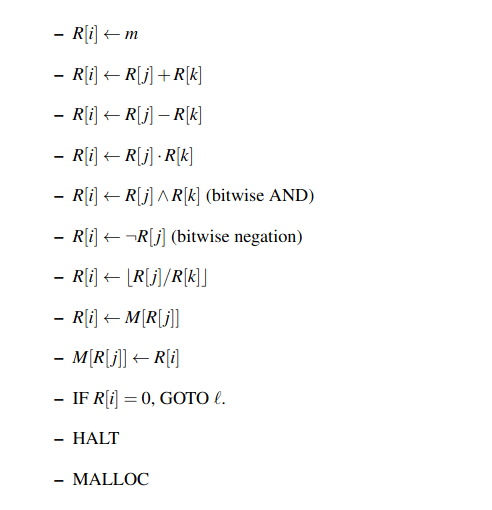
\includegraphics[width=300pt,height=280pt]{slike/instructions_ram.png}

	\caption{Pregled instrukcija u RAM modelu.}	\label{fig: ram_instructions}
\end{figure}

\begin{definition}
   ${w}$-RAM program je bilo koji konačan niz instrukcija $P = (P_1, P_2,\ldots, P_q)$ gore navedenog tipa. Broj $r$ registara je implicitno definiran kao  najveći indeks direktne memorijske adrese (među indeksima $i, j, k$ u skup instrukcija sa Slike~\ref{fig: ram_instructions}) koji se javljaju u programu.
\end{definition}

\subsection{Formalizacija računanja na RAM-u}

Pojam konfiguracije ima za cilj da obuhvati cjelokupno stanje računanja u određenom trenutku --  sve što je neophodno za određivanje budućeg ponašanja.
\begin{definition}
Konfiguracija  \emph{w}--RAM programa $P$ je torka $K = (l, S, w, R, M)$, gdje je $l \in  \{1, \ldots, q + 1\}$ 
programski brojač, $S \in  \mathbb{N}$ je korišteni prostor, $w \in  \mathbb{N}$ je veličina riječi, $R = (R[0], \ldots , R[r - 1]) \in  \{0, \ldots , 2^w - 1\}^r$ je
niz registara, i $M = (M[0], \ldots, M[|S| - 1]) \in  \{0, \ldots, 2^w - 1\}^{|S|}$ je memorijski niz.
\end{definition}
%%https://medium.com/@_SD10_/the-ram-model-of-computation-and-big-o-notation-a1b3cc50ec2c
\begin{definition}
 Za konfiguraciju $K = (l, S, w, R, M)$ \textit{w}-RAM programa $(P_1, \ldots, P_q)$ definišemo sljedeću konfiguraciju $K' = (l', S', w', R', M')$, u zapisu $K$ $\Rightarrow_P K'$, na sljedeći način:
 
 \begin{itemize}
 	\item Ako je $P_l$ = ``IF $R[i] = 0$, GOTO $m$'' za neke $i < r$ i $m \in  \{1, \ldots , q\}$, onda  $K' = (l', S, w, R, M)$ gdje je  $l'= m$ ako je $R[i] = 0$, a $l' = l + 1$ inače. 
 	\item Ako je $P_l$ = ``$R[i] \leftarrow  m$'' za $i < r$, onda $K' = (l  + 1, S, w, R', M)$ gdje  $R'[i] = m$ \emph{mod} $2^w$ i $R'[ j] = R[ j]$ za sve $j \neq i$. 
 	\item Ako je $P_l$ = ``$R[i] \leftarrow R[ j] + R[k]$'' za neki $i, j, k < r$, onda  $K' = (l+1, S, w, R', M)$   gdje je $R'[i] = (R[ j]+R[k])$ \textit{mod} $2^w$
 	i $R'[j] = R[j]$ za sve $j \neq i$.
 	\item Ako je $P_l$ = ``$M[R[ j]] \leftarrow R[i]$'' za $i, j < r$ i $R[ j] < S$, onda $K' = (l+ 1, S, w, R, M')$ gdje je $M'[R[ j]] = R[i]$ i
 	$M'[k] = M[k]$ za sve  $k \neq  R[ j]$.
 	\item Ako je $P_l$ = ``MALLOC'', onda je $K' = (l+ 1, S + 1, w', R, M')$, gdje je $w' = \max\{w, \lceil log_2(S + 1) \rceil \}$, $M'[S] = 0$ i
 	$M'[i] = M[i]$ za $i = 0, \ldots , S-1$.
 	\item Ako je $P_l$ = ``HALT ili  $l = q + 1$'', onda je $K' = (q + 1, S, w, R, M)$.
 \end{itemize}
 
 
\end{definition}

Napomenimo da smo prethodno naveli   samo neke od instrukcija, dok se ostale definišu slično. \\


Definišimo sada formalno pojam računarskog problema shodno prethodno definisanom pojmu RAM modela. 
\begin{definition}
	 RAM program $P = (P_1, \ldots, P_q)$ sa $r \geq 2$ registara rješava problem $f \colon \mathbb{N}^* \rightarrow 2^{\mathbb{N}^* } $
	ako za svaki ulaz $x = (x_1,\ldots, x_n) \in \mathbb{N}^* $ i $k \geq \max\{x_1,\ldots, x_n, m\}$ gdje je $m$ najveća konstanta koja se pojavljuje u $P$, postoji niz konfiguracija $K_0,\ldots,K_t$ tako da:
	\begin{itemize}
		\item $K_0 = (1, n, w, R, M)$ gdje je $w = \lceil \log_2(\max\{n, k +1\})\rceil$, $R[0] = n$, $R[1] = k$, $R[2] = R[3] = \cdots =  R[r-1] = 0$, $M[0] = x_1,
		M[1] = x_2, \ldots , M[n - 1] = x_n$,
		\item $K_{i-1} \Rightarrow_P K_i $ za sve $i = 1, \ldots ,t$,
		\item $K_t = (q+1, S, w, R, M)$ gdje je $(M[1], M[2], \ldots , M[R[0] - 1]) \in  f (x)$. 
	\end{itemize}
\end{definition}

\textit{Komentar}.  Ključne tačke u vezi teorijskog RAM modela su:
\begin{itemize}
	\item  \textit{Ujednačenost}: zahtijevamo da postoji konačan program koji bi trebao raditi za proizvoljne ulaze neograničene veličine
(kad $n, k \rightarrow \infty$).
    \item Računanje se odvija nizom “baznih” operacija.
    \item Ne namećemo a priori ograničenje za vrijeme (broj koraka) ili prostor   (memorija). Ove resurse 
      želimo minimizirati, ali i dalje teorijski RAM model  smatra  algoritmom čak i ako on koristi ogromne količine vremena i prostora, što se, vidjećemo, razlikuje od praktičnog aspekta algoritama. 
\end{itemize}

Pri računanju broja instrukcija izvršavanja programa $P$, u obzir uzimamo sljedeće operacije: aritmetičke i bitske operacije (+, -, *, /, \&, $\mid,\ldots $), logičke ($\wedge$,$\vee$, $\Rightarrow$, $\Leftrightarrow$), operacija dodjele, te ulazno/izlazne operacije. Ove operacije nazivamo \textit{jediničnim instrukcijama}.  Pretpostavka je da se sve jednične instrukcija izvršavaju u jediničnom vremenu.  Vremenska složenost programa se upravo mjeri na osnovu ukupnog broja jediničnih instrukcija, o čemu ćemo više reći u narednoj sekciji. 

\section{Pojam kompleksnosti}

Napomenimo da je jediničnim modelom kompleksnosti definisan (teorijski) RAM model gdje se svaka operacija izvršava u jediničnom vremenu.  Bez obzira što operacije sabiranja i množenja nemaju isto vrijeme izvođenja na stvarnom računaru, to ne umanjuje značaj teorijskog RAM modela, što ćemo prikazati u nastavku.   

Definišimo sada vremensku kompleksnost izvršavanja programa $P$ na RAM modelu.

\begin{definition}
	Vrijeme rada $P$ za ulaz  $x \in \mathbb{N}^*$ je broj $t$ koraka prije nego $P$ dostigne zaustavnu
	konfiguracija (operacija ``HALT'') za $x$. Dakle, najmanji $t$ za koji postoji niz $K_0 \Rightarrow_P  K_1 \Rightarrow_P \cdots \Rightarrow_P K_t$ takav da je $K_0$
	početna konfiguracija od $P$ za ulaz $x$, a $K_t$ je konfiguracija zaustavljanja (gdje se programski brojač  ažurira na $q + 1$, a $q$
	označava broj instrukcija u programu $P$).  
	Pogledajmo sljedeći primjer. 
	
\end{definition}
 
%\begin{example} \\
	
\begin{minted}{C}
	algoritam max(a, n)
	  maximum = a[0]
 	  for i in 1 to n-1 do
	      if a[i] > maximum then
                  maximum = a[i]
          return maximum    
\end{minted}

%\end{example}

Izračunajmo tačan broj instrukcija programa konkretnog ulaza $a = [1\ 5\ 2\ 10\ 7]$ i $n = 5$. Imamo: prva linija sadrži jednu instrukciju (dodjela). Unutar petlje (koja se izvršava $n-1$ puta, za koju se dodjeljuje nova  vrijednost iteratoru \texttt{i}, te se potom provjerava da li je ona veća od $n$), broj instrukcija koji je uvjetovan prolazom elementima niza  $\texttt{a}$ je $5, 3, 5$ i $3$, što je ukupno $1+5+3+5+3=17$ izvršenih instrukcija.  U kombinaciji sa instrukcijama za varijable \texttt{i} u \emph{for} petlji, ovaj program izvršava ukupno $17+ 4 \cdot 2 + 1 = 26$ instrukcija.



Vremenska složenost izvršavanja programa se mjeri u odnosu na ukupan broj
jediničnih instrukcija. Tačan broj instrukcija za svaki ulaz u kompleksnim programima je     teško precizno izračunati. Zbog toga uvodimo pojam \textit{najgoreg vremena izvršavanja} programa (eng. \textit{worst-case running time}) koji nam pruža   lakši način računanja broja instrukcija programa, ali opet dovoljno reprezentativan da ukaže na to koliko je algoritam efikasan. 

\begin{definition}
	  Najgore vrijeme izvršavanja programa $P$ je funkcija $T \colon \mathbb{N} \times \mathbb{N} \rightarrow \mathbb{N}$ gdje je $T (n, k)$ maksimalno
	vrijeme rada programa $P$ u odnosu na sve moguće ulaze $x \in  \{0, \ldots , k\}^n$.
\end{definition}

\begin{example} 
	
	Pogledajmo sljedeći program  \\  \vspace{0.3cm} 
\begin{minted}{Python}

algoritam sort(a, n)
  for i in 1  to n-1 do
     for j in 0 to  i-1 do
        if a[i] > a[j] then
           swap (a[i], a[j])
           
           	\end{minted}
\end{example}

Najgori slučaj za ulazne podatke je kada se instrukcije pod \emph{if}--petljom stalno izvršavaju; to je slučaj kada je na ulazu niz \texttt{a} kojem su elementi poredani u obrnutom  poretku u odnosu na traženi poredak. Prema tome \texttt{swap} operacija se tada izvršava u svakoj iteraciji, i ona sadrži 3 instrukcije (dodjela). Unutrašnja petlja se izvršava $i$ puta  za svaki $i=1, \ldots, n-1$.  Tada imamo da je  
$$ \sum_{i=1}^{n-1} \sum_{j=0}^{i-1} 2 \cdot 3 = 6 \sum_{i=1}^{n-1} i = 3 \cdot {(n-1) \cdot n}$$ najveći (najgori) broj instrukcija koji algoritam izvršava za svaki ulaz dužine $n$. 
\\


Za najgore vrijeme izvršavanja  uzimamo najgori slučaj ulaznih podataka određene dimenzije za koji će se izvršiti maksimalan broj instrukcija. Motivacija za računanje najgoreg vremena izvršavanje programa (algoritama) je sljedeća. Najgori slučaj izvršavanja algoritma je obično lakši za detektovanje i izračunavanje nego je to slučaj sa   tačnim brojem koraka (instrukcija) za konkretnu instancu, koji ne govori mnogo o broju instrukcija programa za ulaze drugačijih distribucija. Prepoznavanje najgoreg slučaja za ulazne podatke određene dimenzije za koje program radi najduže nam omogućuje da utvrdimo gornju granicu za broj instrukcija svakog mogućeg izvršenja programa. Ovakvo vrijeme izvršavanja ne  zavisi od konkretne (distribucije) ulazne instance, čime se dobija bolji osjećaj o efikasnosti programa u odnosu na veličinu ulaza.
 
Bez obzira na ovakva pojednostavljenja, i dalje je egzaktno računanje najgoreg vremena izvršavanja težak posao u većini kompleksnih programa. Stoga, u nastavku govorimo o pojmu \textit{asimptotskog} vremena izvršavanja programa.  Gotovo uvijek se broj koraka izvršavanja u algoritmu povećava shodno povećavanju dimenzije ulaza. Prema tome, ima smisla posmatrati ponašanje algoritma na  
ulazima velike dimenzije jer se često programi čiji su ulazi  malih dimenzija ionako efikasno izvršavaju (imaju kratko vrijeme izvršavanja)  nezavisno od algoritamske tehnike rješavanja. U sljedećoj podsekciji, formalno uvedimo pojam $O$--notacije. 
 
 
\subsection{$O$--notacija} 
$O$-notacija   dodatno pojednostavljuje ocjenjivanje broja izvršenih instrukcija  programa, fokusirajući se na ponašanje algoritma na ulazima velikih dimenzija.  Pretpostavimo da imamo sljedeću situaciju o ocjeni najgoreg scenarija izvršavanja dva algoritma (na istom posmatranom problemu): 
\begin{itemize}
	\item $T_1(n) = 2 n^{\frac{3}{2}} + 3n + 10$
	\item $T_2(n) = 4 n \cdot \log n + \lceil \sqrt{n} \rceil + 22 $
\end{itemize}

Upoređivanje ovakvih funkcija zahtjeva analitičku analizu obje funkcije, pri čemu se može utvrditi da je prvi algoritam (koji se izvršava u $T_1$ vremenu u odnosu na ulaz veličine $n$)  brži -- zahtjeva izvođenje manjeg broja instrukcija -- za manje $n$, dok je za veće $n$ očigledno u prednosti algoritam sa vremenom izvršavanja $T_2$ ($n \log n$ dosta sporije raste od funkcije $n^{\frac{3}{2}}$). 

Dakle, cilj je je pojednostaviti računanje izvršenog broja instrukcija, koje se postiže uvođenjem sljedećih konvencija u svrhu ocijenjivanja ponašanja algoritma na instancama velikih dimenzija.
\begin{enumerate}
	\item Konstante uz svaki od termova se ignorišu.
	\item Dominantni termovi se uzimaju, dok se ostali (nedominirajući) ignorišu. Dominantan je onaj term koji najbrže raste sa porastom dimenzije ulaza. Dakle, procjenjuje se asimptotsko ponašanje broja instrukcija u zavisnosti od veličine ulaza programa. 
\end{enumerate}

Za $T_1(n)$  je dominantni term funkcija $n^{\frac{3}{2}}$, dok je to za $T_2(n)$ funkcija $n \cdot \log n$. 
 
 Nadalje pretpostavimo da radimo sa pozitivnim funkcijama, sa pozitivnim vrijednostima argumenata. 

%%https://www.khanacademy.org/computing/computer-science/algorithms/asymptotic-notation/a/big-o-notation

\begin{definition}
Neka su date dvije funkcije $f$ i $g$. Kažemo da $f = O(g)$ akko postoji konstanta $c >0$ tako da $f(n) \leq c \cdot g(n)$ počevši od nekog dovoljno velikog $N$. tj. za $n \geq {N}$. Kažemo da je $g$ (gornja) asimptotska granica za $f$. 
\end{definition}

\begin{figure}[H]
	\centering
	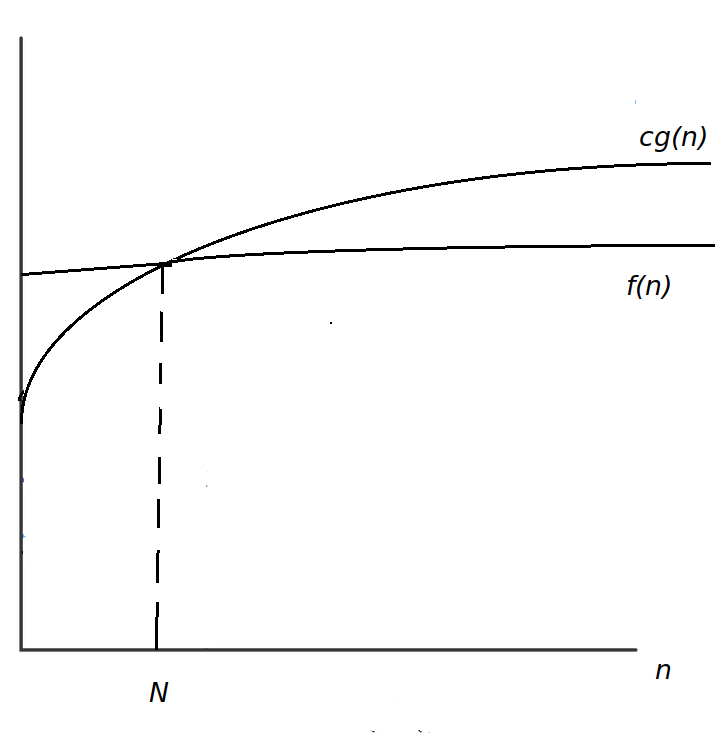
\includegraphics[width=120pt,height=110pt]{slike/O_notation.png}
	\label{fig:O_notation}
	\caption{$O$--notacija: vizuelizacija.}
\end{figure}


%https://afteracademy.com/blog/time-and-space-complexity-analysis-of-algorithm/

\begin{example}
	Jasno je da $T_1 = O(n^2)$, ali i $T_1 = O(n^{\frac{3}{2}})$ Takođe, $T_2 = O(n \log n)$. 
\end{example}

U osnovi, dominirajući term nam govori o asimptotskoj granici čitavog izraza (dobijen računanjem (najgoreg mogućeg) broja instrukcija izvršenog u programu), jer kad je $n$ dovoljno veliko, vrijednost izraza dominantno zavisi od dominirajućeg terma, dok se ostali termi doprinose u ne tako značajnoj mjeri da bi se promijenio zaključak o asimptotskom ponašalju porasta broja instrukacija programa sa porastom dimenzije ulaza. 

$O$--notacija, bez obzira na praktičnost i jednostavnost, dovodi i do određenih  dvosmislenosti. Npr.\  $n^2 + n = O(n^2)$, ali vrijedi i $n^2 + n = O(n^3)$. U svakom slučaju, korisniji zaključak dobijamo uzimajući prvi od ova dva.  Ovo nas dovodi do definisanja $\Theta$--notacije (eng. Big-Theta).

\begin{definition}
Neka su date dvije funkcije $f$ i $g$.  Ako $f = \Theta(g)$, onda postoje konstante $c_1, c_2 >0$ tako da $c_1 g(n) \leq f(n) \leq c_2 g(n)$, počevši od nekog dovoljno velikog $n$. 
\end{definition}

U prevodu, funkcije $f$ i $g$ imaju isto asimptotsko ponašanje (dakle, za velike vrijednosti ulaza $n$), vidjeti Sliku~\ref{fig:theta_notation}. 

\begin{figure}[H]
	\centering
	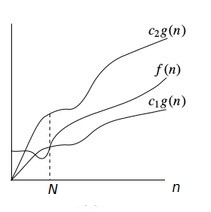
\includegraphics[width=120pt,height=120pt]{slike/theta_notation.jpg}
 
	\caption{$\Theta$--notacija: vizuelizacija.}	\label{fig:theta_notation}
\end{figure}

\begin{example}
Imamo	$T_1 = \Theta(n^{\frac{3}{2}})$, dok je $T_2 = \Theta(n \log n)$.  
\end{example}

Postoji još nekoliko notacija za kompleksnost algoritama, a to su $\Omega$ i $o$--notacija.

\begin{definition}
 Neka su date dvije funkcije $f$ i $g$. Kažemo da $f = \Omega(g)$ akko postoji konstanta $c >0$ tako da je $f(n) \geq c g(n)$, počevši od nekog dovoljno velikog $n$.  
\end{definition}
$\Omega$-notacija govori o funkcijama za koje je $g$ asimptotska donja granica, budući da ograničava rast vremena rada odozdo za dovoljno velike veličine ulaza.

\begin{example}
  Vrijedi $n^3= \Omega(n^2 + n)$ i $n\log n = \Omega(n)$.
\end{example}

\begin{definition}
	Neka su date dvije funkcije $f$ i $g$. Kažemo da $f = o(g)$ akko za sve $c > 0$ postoji   $N > 0$ takav da je $0 \leq f(n) < cg(n)$ za sve $n \geq N$. 
	
\end{definition}

\noindent \textbf{\textit{Napomena}}. Vrijednost $k$ ne smije zavisiti od $n$, ali može da zavisi od $c$.

Neformalno, ako $f(n) = o(g(n))$, to znači da  $f$ postaje beznačajno mala u odnosu na $g$ kako se $n$ približava beskonačnosti.

\begin{example}
    Vrijedi $n = o(n^2)$, kao i $n = o(n^3)$, ali ne vrijedi $n = o(n)$. 
\end{example}

\subsection{Neka svojstva $O$--notacije}

\begin{theorem} Neka su $f, g$ i $h$ pozitivne funkcije, pozitivnih vrijednosti argumenata.  Vrijede sljedeće tvrdnje:
	\begin{itemize}
		\item 	  $f = O(c \cdot f)$ za svako $c > 0$ (konstantni faktori su irelevantni);
		\item Ako $f = O(g +  h)$ i $h = O(g)$, onda je i $f = O(g)$  (pravilo dominantnog terma);
		\item $O(f + g) = O(f)  + O(g)$ (pravilo zbira);
		\item $O( f \cdot g) = O(f) \cdot O(g)$ (pravilo proizvoda);
        \item $f = O(g)$ i $g = O(h)$ onda
        vrijedi i $f = O(h)$ (pravilo tranzitivnosti). 
	\end{itemize}
 
\end{theorem}

\begin{proof}
	Dokazi tvrdnji se direktno izvode na osnovu definicije $O$--notacije.
\end{proof}

\subsection{Uputstva za procjenu kompleksnosti algoritama}

Prethodna sekcija nam daje na uvid neke od osnovnih notacija za ocjenjivanje kompleksnosti   algoritma, tj. izvršenja broja instrukcija programa koja se obično razmatra u zavisnosti od veličine ulaza. 

 Najčešće funkcije koje se pominju u analizi kompleksnosti izvršavanja algoritama su nabrojane u Tabeli~\ref{tab:kompleksnosti}. 
 
 \begin{table}[H]
 	   \caption{Rast funkcija. }  \label{fig:kompleksnosti_funkcije}
 	\centering 
 	\begin{tabular}{l |l} \hline 
 		\textbf{Funkcija}   & \textbf{Kompleksnost} \\ \hline
 		1          & konstantna \\
 		$\log n$   & logaritamska \\
 		$n$        &  linearna \\
 		$n \log n$ & super-linearna  \\
 		$n^2$      & kvadratna \\
 		$n^3$      & kubna \\
 		$2^n $     & eksponencijalna \\ 
 		$n!$       & faktorijel \\
 		\hline
  	\end{tabular}

 \end{table}
 Rast svake od ovih funkcija sa porastom ulaza ($n$) je prikazan na Slici~\ref{fig:kompleksnosti_funkcije}
 \begin{figure}[H]
 	\centering
 	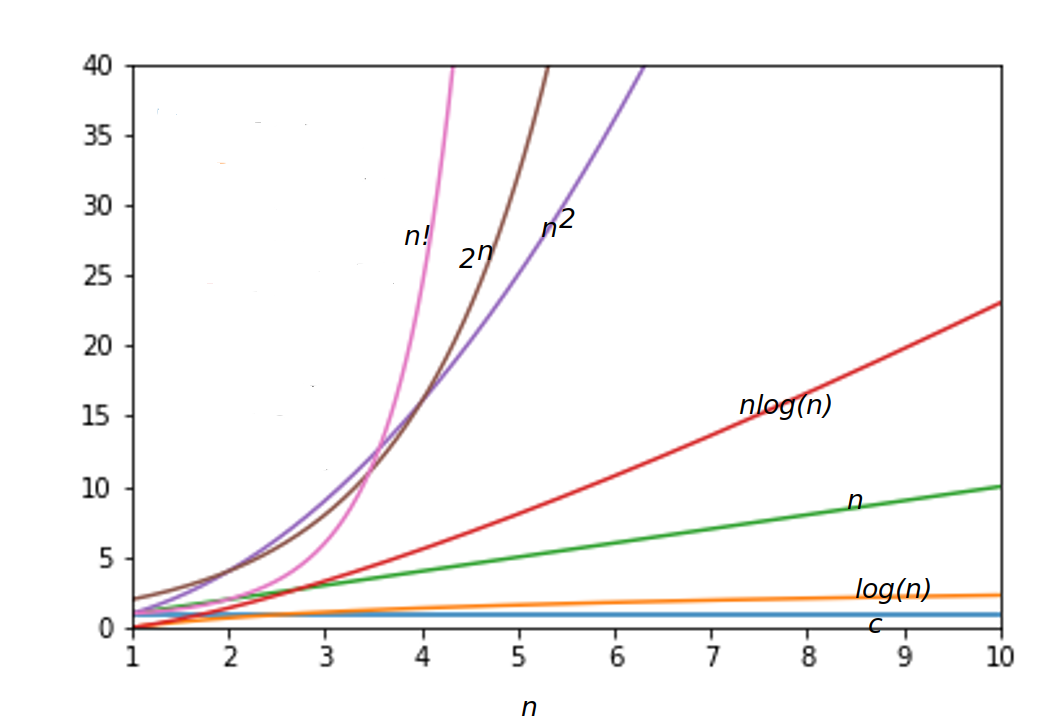
\includegraphics[width=270pt,height=200pt]{slike/growth.png}%growth-Functions.jpg}
   \caption{Rast funkcija. }  \label{fig:kompleksnosti_funkcije}
 \end{figure}


U praksi, neželjena kompleksnost algoritma je eksponencijalna, dok su logaritamska, linearna i log-linearna kompleksnost poželjne i takvi algoritmi su obično veoma efikasni u rješavanju problema, tj. instanci velikih dimenzija. U zavisnosti od tipa problema, kvadratna kompleksnost može ali i ne mora biti garant za rješavanje realnih instanci većih dimenzija razmatranog  problema. %U najvećem broju slučajeva, klasa funkcija koja  koja prelazi kvadratnu je nedovoljno dobra. 


U nastavku izlažemo neka uputstva koja olakšavaju računanje kompleksnosti algoritma. Za (pod)program $P$, označimo njegovu kompleksnost izvođenja sa funkcijom $T(P)$ koja (direktno ili indirektno) zavisi od dimenzije ulaza ($n$). 
 
\begin{table}[H]
		\caption{Uputstva za računanje kompleksnosti algoritma.}  \label{tab:uputstva_racunanje}
	\centering
	\begin{tabular}{l |l} \hline 
		\textbf{Konstrukcija}         & \textbf{Računanje kompleksnosti} \\ \hline
		Jedinične instrukcije         & 1 \\
        Serija naredbi $S$: $N_1$; $N_2$; &  $T(S) = T(N_1) + T(N_2)$  \\ \hline
        Naredba grananja $S$:           &                                \\
        \textbf{IF}  $C$ then $N_1$ \textbf{ELSE} $N_2$  & $T(S) = T(C) + \max\{ T(N_1), C(N_2)\}$  \\          \hline                 
         Naredba petlje $S$:            &   $n$ -- maksimalan broj iteracija          \\
         1) \textbf{WHILE} $U$ \textbf{DO} $N_1$                 &     $T(S)= n \cdot (T(U) + T(N_1))$         \\ 
         2) \textbf{FOR} $i=j$ \textbf{to} $p$ \textbf{DO} $N_1$  &    $T(S)= n\cdot T(N_1)$     \\  \hline
         
	\end{tabular}
\end{table}

Odgovorimo sada na pitanja da li je jedan algoritam efikasniji od drugoga?
Upravo, odgovor nam daju notacije za kompleksnost koje smo naučili u ovoj glavi, i to dvije najznačajnije: $O$ i $\Theta$--notacije. Kažemo da je jedan algoritam $X$ \textit{asimptotski efikasniji} od drugog algoritma  $Y$ akko sa porastom veličine ulaza u oba algoritma, vrijeme rada algoritma $X$ postaje kraće od vremena rada $Y$. To znači da $X$ pripada nižoj $O$--klasi složenosti od $Y$. %https://www.geeksforgeeks.org/algorithms-analysis-of-algorithms-question-16/ 
Prema tome, za velike ulaze, algoritam $X$ je uvijek biti bolji izbor od  algoritma $Y$ u smislu efikasnosti (vremena izvođenja). Međutim, za male ulaze moguće je da je $Y$ i dalje brži od $X$. Stoga se ne može reći da je $X$ uvijek bolji izbor za sve ulazne vrijednosti, već da će $X$ biti bolji izbor za sve ulaze osim eventualno malih ulaza.


U narednom primjeru dajemo jedan zadatak, rješavamo ga na dva načina, te izvodimo kompleksnost oba programa.

\begin{example}
 \textit{{Problem nalaska (neprekidnog) podniza  maksimalne sume}}.  Od svih neprekidnih podnizova datog
 niza, naći onaj čija je suma elemenata najveća moguća. 
\end{example}
\begin{solution}
 
 Neka je dat ulaz $\texttt{a} = [1, 4, -2, 2, 10, -7, 1]$.  Jedan neprekidan podniz ovog niza je $[ -2, 2, 10 ]$ (početne pozicije 2, te završne pozicije 4), ali $[-2, -7, 10]$ nije neprekidan podniz. 
 
Koristimo se naivnim pristupom rješavanja problema. Definišimo $$S(i, j) := \max  \{ a[i], \ldots, a[j] \},$$

gdje je $S(i, i ) = a[i]$. 
Funkcija $S(i,j)$ računa sumu elemenata neprekidnog podniza niza \texttt{a}, sa početnom pozicijom  $i$, te završnom pozicijom $j$.
Za izračunavanje funkcije $S(i, j)$, potrebno je $j-i+1$ instrukcija, što definitivno pripada klasi $O(n)$. Da bismo riješili problem na ovaj način, 
treba da pozovemo funkciju $S(i,j)$ za svaki par $(i,j),  {i, j \in \{0, \ldots , n-1\},  i \leq j}$, a to je ukupno $\binom{n}{2} + n$ puta, što odgovara klasi kompleksnosti $O(n^2)$. Dakle, kompleksnost ovakvog algoritma je $O(n)\cdot O(n^2) = O(n^3)$ što je kubna kompleksnost. 

Pokušajmo konstruisati ``pametniji'' algoritam. Iskoristimo činjenicu da postoji jasna rekurzivna zavisnost između vrijednosti dva susjedna $S(i,j)$ i $S(i, j+1)$, tj. da je $S(i, j+1) = a[j+1] + S(i, j)$, za $j \in \{i, \ldots, n-2\}$. Definišimo sada:
$$ S(i):= \max \{ S(i, i), S(i, i+1), \ldots, S(i, n-1)\}.$$

Izvršavanje funkcije $S(i)$ se odvija u linearnoj kompleksnosti, tj. $O(n)$. Kako se ona poziva $n$ puta (za svako $i \in \{0, \ldots n-1\}$ po jednom), ukupna kompleksnost ovog pristupa je $n \cdot O(n) = O(n^2)$, što je znatno efikasnije od prethodnog, naivnog, pristupa. 
 

\end{solution}



 
 
 \section{Prostorna kompleksnost}
 
 %https://www.geeksforgeeks.org/g-fact-86
 
 Termin prostorna kompleksnost se na mnogim mjestima pogrešno koristi asocirajući na pomoćni prostor.  \textit{Pomoćni prostor} je dodatni ili privremeni prostor koji koristi algoritam.
 
 \textit{Prostorna složenost} algoritma je ukupan prostor koji algoritam zauzima u odnosu na veličinu ulaza. Prostorna složenost   uključuje i pomoćni prostor i prostor koji koristi ulaz.
 
 Prostorna složenost se može posmatrati kao pandan koncepta vremenske složenosti. Za kreiranje niza veličine $n$, zahtijeva se dodatan prostor od $O(n)$. Za kreiranje dvodimenzionalnog niza veličine $n \times n$,  zahtijeva se $O(n^2)$ prostora.
 Napomenimo da prostorna kompleksnost zavisi i od programskog jezika, kompajlera, pa  čak i mašine koja pokreće algoritam.
 
 
 Efikasnost algoritma uglavnom je definisana u odnosu na  dva faktora, korišteni prostor i vrijeme. ``Dobar'' algoritam je onaj koji koristi manje vremena i prostora; međutim, to nije moguće stalno postići. Zbog toga postoji kompromis između vremena i prostora. Ako želimo skratiti vrijeme izvršavanja algoritma, korišteni prostor se obično povećava. Slično tome, ako želimo smanjiti prostor, vrijeme izvršenja algoritma se obično povećava. %Dakle, treba napraviti kompromis između prostora i vremena.  
 
 
 \begin{example}
 	Posmatrajmo sljedeći pseudokod, te odredimo prostornu kompleksnost datog 
 	programa. 
 	
 	
 	\begin{algorithm}[H]
 		\begin{algorithmic}[1]
 			\Procedure{pairSum}{x, y}   
 			\State	\textbf{return} $x+y$
 			\EndProcedure
 			
 		\end{algorithmic}
 	\end{algorithm}        
 	
 	
 	\begin{algorithm}[H]
 		\begin{algorithmic}[1]
 			\Procedure{addSequence}{n}
 			
 			\State $sum \gets 0$
 			\For{$i = 0 \text{ to } n-1$}
 			\State $sum \gets sum + \texttt{pairSum}(i, i+1)$
 			\EndFor
 			\State \textbf{return} \textit{sum}~
 			\EndProcedure
 			
 		\end{algorithmic}
 	\end{algorithm}
 	
 	Prostorna kompleksnost procedure \textsc{AddSequence} je jednaka $O(1)$, bez obzira što se funkcija \textsc{pairSum} poziva $O(n)$ puta. Zašto?
 	
 	
 \end{example}
 
 
  \textbf{\textit{Napomena}}. U standardnom programiranju, podrazumijeva se korištenje 256MB prostora za određeni program. Dakle, kreiranje   niza veličine veće od $10^8$ nije dozvoljeno, jer je na raspolaganju data gornja granica za količinu memorije na  raspolaganju. Takođe, kreiranje  niza veličine veće od $10^6$ u tijelu funkcije nije moguće, jer je maksimalni prostor dodijeljen funkciji (u lokalnom steku) 4MB. Dakle, da bismo koristili niz veće veličine, potrebno je kreirati globalni niz.

\section{Pseudokod}

\textit{Pseudokod} je jednostavan prikaz implementacije algoritma u obliku anotacija i informativnog teksta napisanog na običnom jeziku. On nema sintaksu kao bilo koji programski jezik i stoga ga računar ne može kompajlirati ili interpretirati. % Često su algoritmi  predstavljeni pomoću pseudo kodova jer se mogu protumačiti bez obzira na znanje onog koji ga nasoji razumjeti. 
 Pseudokod, kao što sam naziv sugeriše, je reprezentacija k\^oda koja je prilagođena da ga razumiju i osobe bez velikog znanja o programiranju i algoritmima. Za razliku od pseudokoda, algoritam je organizirani   niz instrukcija koji rješava određen problem pri implementiranju u nekom programskom jeziku, te se kompajliranjem  ili interpretiranjem prevodi u mašinski k\^od kojeg mašina može da izvrši.

Prednosti korištenja pseudokoda su sljedeće. 
\begin{itemize}
	\item Poboljšava čitljivost i razumijevanje bilo kojeg pristupa kojim se rješava problem.
%	\item Predstavlja jedan od najboljih načina za  implementaciju algoritma.
	\item Djeluje kao spona između programa i dijagrama toka.
	\item Služi kao gruba dokumentacija, da bi se program mogao lakše razumjeti. U industriji je vođenje dokumentacije od suštinskog značaja i tu se potreba za pseudokodom pokazuje krucijalnim.
\end{itemize}
 
 
Glavni cilj pseudokoda je da nedvosmisleno objasni suštinu svakog dijela programa, čime se olakšava faza izgradnje k\^oda te smanjuje mogućnost pravljenja  grešaka u implementaciji algoritma.

Pisanje pseudokoda počinje razumijevanjem problema koji se rešava. Nakon  jasnog definisanja problema, slijedi razmatranje koraka koje treba preduzeti kako bi se došlo do rešenja. Te korake zatim zapisujemo uz pomoć  pseudokoda.

Nekoliko saveta u vezi prakse pisanja ``dobrog''  pseudokoda su:
\begin{itemize}
	\item Koristiti jasne i precizne nazive za promenljive i funkcije.
	\item Koristiti opise koji jasno ukazuju na to šta se dešava u svakom koraku algoritma. 
	\item Razmisliti o slučajevima u kojima algoritam može da se zaustavi i načinima na koje  se to može desiti.
	\item Koristiti odgovarajuće sintakse za kontrolne strukture kao što su petlje i uslovi: \texttt{if-else}, \texttt{for}, \texttt{while} petlje. Koristiti mehanizam uvlačenja naredbi koje se izvršavaju u okviru istog bloka, jer pomaže lakšem shvatanju kontrolnog mehanizma i izvršavanja odluka. Ovakva praksa u velikoj mjeri poboljšava čitljivost k\^oda. Pogledajmo u nastavku primjer jednog jednostavnog pseudokoda.
	
	\begin{minted}{C}
        
                tip = unos sa tastature
		if tip == "1"
		   ispiši odgovor "Unesen je broj 1"
		
		if tip == "2"
		   ispiši odgovor "Unesen je broj 2"
	\end{minted}
	
	\item Dakle, pseudokod nije potrebno pisati na potpuno programski način. Njegova svrha je jednostavnost i razumijevanje čak i za osobe kojima programiranje nije struka, stoga ne bi trebalo sadržati previše tehničkih detalja.
\end{itemize}

\begin{example} Napisati pseudokod za nalazak najvećeg elementa u nizu. \\
 \begin{minted}{C}
 Inicijalizuj najveći broj na prvi element niza.
 Proći sve preostale elemente niza: 
    Ako je trenutni element veći od trenutno najvećeg broja,
    postavi trenutni element kao novi najveći broj.
 Kraj petlje.
 Ispiši najveći broj.
 \end{minted}
 
\end{example}

U nastavku navodimo (koncizniji) pseudokod, koji rješava problema nalaska podniza  maksimalne sume na efikasniji način. Ovdje će biti korišten česten format koji je više tehnički, a i više upotrebljavan u literaturi. 
 
 

 \begin{algorithm}[!ht]
 	\caption{Funkcija $S_i(i)$}\label{S_i}
 	\begin{algorithmic}[1]
 		\Procedure{S}{$i$, $niz$}
 		\State $s_{maxi}, s_{next} \gets niz[i]$
 		\For{$j=i+1$ to $n-1$}
 		\State $s_{next} \gets s_{next} + niz[j]$
 		\If{$s_{next} > s_{maxi}$}
 		\State $s_{maxi} \gets s_{next}$
 		\EndIf
 		\EndFor  
 		\State \Return $s_{maxi}$
 		\EndProcedure
 	\end{algorithmic}
 \end{algorithm}



\begin{algorithm}[H]
	\caption{Funkcija $S$}\label{S}
	\begin{algorithmic}[1]
		\Procedure{S}{$niz$}
		\State $s_{max}\gets niz[0]$ 
		\For{$i=0$ to $n-1$}
		\State $s_i \gets  S_i(i)$ 
		  \If{$s_{max} <  s_{i}$}
		    \State $s_{max} \gets s_{i}$
		  \EndIf
		\EndFor  
		\State  \Return  $s_{max}$
		\EndProcedure
	\end{algorithmic}
\end{algorithm}

\section{O valjanosti algoritma}

Postoji nekoliko načina da se formalno provjeri valjanost algoritama; tri  su osnovna načina:

\begin{itemize}
	\item \textit{Matematički dokaz}. Predstavlja jedan od najrigoroznijih načina za provjeru valjanosti algoritma.  %je matematički pokazati da algoritam uvijek daje ispravan izlaz. 
	Ovdje se koriste matematičke tehnike za analizu logike algoritma i za utvrđivanje da algoritam radi ispravno za sve moguće ulaze. Jedana od metoda je \textit{metoda invarijantne petlje}, kojom ćemo se pozabaviti u nastavku ove sekcije. 
	
    \item \textit{Formalna verifikacija}. Formalna verifikacija je proces upotrebe matematičkih tehnika i alata za provjeru da li algoritam ispunjava određene specifikacije. Ovo uključuje modelovanje algoritma korištenjem formalnog jezika, a zatim korištenje automatiziranih alata za provjeru da li model zadovoljava određena svojstva. U osnovi, ovi metodi su iz domena vještaške inteligencije specijalno namijenjeni za verifikaciju softvera.
    \item \textit{Testiranje}.  Iako testiranje nije formalna metoda već \textit{empirijska}, ona predstavlja važan način za provjeru valjanosti algoritma. Pokretanjem algoritma sa raznim ulaznim vrijednostima i provjeravanjem izlaza u odnosu na očekivane rezultate, može se steći povjerenje o tome da li je algoritam ispravan.

\end{itemize}


Metoda \textit{invarijantne petlje} (eng. \textit{{loop} {invariant}}) predstavlja jednu od matematičkih tehnika koja se koristi u dokazivanju ispravnosti algoritama. Invarijanta petlje je tvrdnja koja ostaje istinita tokom svake iteracije petlje programa, uključujući i prije i poslije izvršavanja naredbi u iteraciji.

Da bismo koristili metod invarijantne petlje u dokazivanju ispravnosti algoritma, najčešće se kombinuju sljedeći koraci.

\begin{itemize}
	\item  Definisanje invarijante petlje: potrebno je definisati tvrdnju koja ostaje istinita prije i poslije svake izvršene iteracije petlje.
   \item Dokazivanje inicijalne invarijante: treba pokazati da je invarijanta petlje istinita prije prve iteracije petlje.
   \item Dokazivanje održavanja invarijante: potrebno je dokazati da ako je invarijanta istinita prije određene iteracije petlje, onda je istinita i nakon izvršavanja te iteracije.
   \item Dokazivanje da se petlja završava: pokazati da se nakon konačnog broja iteracija, petlja prekida.
   \item Dokazati da algoritam rješava problem: potrebno dokazati da, ako je invarijanta istinita, nakon posljednje iteracije petlje, algoritam uistinu rješava problem.
\end{itemize}

Ova metoda je korisna u dokazivanju ispravnosti algoritama koji se sastoje od petlji, jer omogućava dokazivanje da algoritam radi ono što je i očekivano, tj. da ispravno rješava problem za sve moguće ulaze.

\begin{example}
Demonstrirajmo   pokazivanje ispravnosti programa za nalazak \textit{najvećeg zajedničkog djelioca (NZD)} dva prirodna broja, datog   Algoritmom~\ref{alg:nzd}, uz pomoć metoda invarijantne petlje.


\begin{algorithm}
	\begin{algorithmic}[1]
		\Procedure{NZD}{$n, m$}
		\State $nzd \gets \min(n, m)$
		\While{!($n \% nzd == 0 \  \& \ m \% nzd == 0$)}
		    \State $nzd \gets nzd - 1$
		\EndWhile
		\State \Return $nzd$
		\EndProcedure
	\end{algorithmic}
   \caption{NZD dva broja.} \label{alg:nzd}
\end{algorithm}

Ovaj program je konačan, jer je broj iteracija u glavnoj \emph{while}-petlji najviše $nzd$, dok je broj instrukcija u svakoj iteraciji takođe konačan (jednak 5+2=7). Dalje, odredimo uslov invarijantne petlje. Neka je ${nzd}^*$ konačan rezultat koji program vraća (koji je zasigurno zajednički djelilac, po uslovu prekida petlje). Tada  invarijantnu petlju definišemo sa 
$$ nzd^* \leq nzd.$$

Prije ulaska u prvu iteraciju petlje imamo $nzd^* \leq nzd = d_0 = \min(n, m)$. 
Neka je prije ulaska u $k$-tu iteraciju petlje $d_{k-1} = nzd$. Tada je  $nzd^* < d_{k-1}$ jer se  ulaskom u $k$-tu iteraciju petlje uvjeravamo da $d_{k-1}$ ne može biti NZD ulaznih brojeva (jer tada zadovoljava uslov \textit{while}-petlje). Tada imamo $d_{k} = d_{k-1} -1 \geq nzd^*$ nakon završetka $k$-te iteracije, čime je uslov invarijantne petlje i tada zadovoljen.   Pretpostavimo da se u iteraciji $k^*$ program prekida. To znači da je $d_{k^*-1}$ zasigurno zajednički djelilac. Kako tražimo najveći takav, onda je i $d_{k^*-1} \leq nzd^*$. S obzirom da je  $d_{k^*-1} \geq nzd^*$ zbog uslova invarijantne petlje, slijedi da je 
$d_{k^*-1} = nzd^*$, čine smo pokazali valjanost algoritma.
\end{example}
Pokazivanje valjanosti kompleksnih algoritama pomoću metoda invarnijantne petlje je rijetko  praktično. Jedan od razloga je taj što definisanje samog uslova invarijantnosti nije trivijalan zadatak, kao  i to da instrukcije koje se izvršavaju u svakoj iteraciji nisu trivijalne  (kao što je to slučaj sa prethodnim programom), te mogu uključivati  pozivanje složenijih pomoćnih funkcija. U takvim slučajevima, valjanost algoritma provjeravamo empirijski, izvršavajući ga nad instancama različitih veličina i distribucija te provjeravajući  validnost vraćenih rezultata (za instance za koje znamo tačan rezultat, dok za one za koje ne znamo, provjeravamo ispunjivost uslova zadatka). 

\section{Euklidov algoritam: kompleksnost}
Klasični algoritam za nalazak NZD je Euklidov algoritam, dat Algoritmom~\ref{alg:nzd-euclid}. On predstavlja jedan od najpoznatijih algoritama u polju aritmetike. Izvedimo njegovu vremensku kompleksnost. 

\begin{algorithm}
	\begin{algorithmic}[1]
		\Procedure{NZD}{$p, q$}  \# pretpostavka je da $p \geq  q$
		\State $x \gets p$ 
		\State $y \gets q$
		\While{ $y > 0 $}
		\State $ x \gets y  $
		\State $y \gets x \% y $
		\EndWhile
		\State \Return $x$
		\EndProcedure
	\end{algorithmic}   \caption{NZD dva broja.} \label{alg:nzd-euclid}
\end{algorithm}

\begin{solution}
	Prvo izvedimo korake algoritma na konkretnoj instanci. Neka je $p=400$, a $q=24$. Tada imamo korake:
	$$(400, 24) \rightarrow (24, 16) \rightarrow (16, 8) \rightarrow (8, 0),$$
	odakle slijedi da je NZD$(400, 24)=8$. Za razliku od naivnog algoritma za nalazak NZD iz prethodnog poglavlja, koji bi za ovu instancu izveo 17 iteracija do nalaska rješenja, vidimo da za Euklidov algoritam treba svega 4 iteracije da nađe tačno rješenje. 
	
	Prvo, Euklidov algoritam je konačan, jer je broj iteracija ograničen sa $\min(p, q)$. Drugo, algoritam ne zavisi direktno od veličine ulaza (koji je konstantan, tj. veličine $2=|\{p, q\}|$), već od veličine brojeva, ili dužine binarne reprezentacije (dekadnih) brojeva u ulazu. Ako je $p$ broj u dekadnom zapisu, dužina njegovog binarnog zapisa jednaka je $\lfloor \log_2(p) \rfloor+1$. Dalje, označimo sa $n_1$   broj bitova u zapisu broja $p$, a sa $n_2$  broj bitova u zapisu broja $q$. 
	Tada je
	$$n_1 \approx \log_2(p), n_2 \approx \log_2(q),  n = n_1 + n_2 = \log_2(p \cdot q ).$$
	
	Vrijednost $n$ je najveća kada su $p$ i $q$ susjedni brojevi, odakle je $ n_1 \approx n_2 \approx n/2$,  pa za kompleksnost algoritma $T(n)$ vrijedi da je proporcionalna vrijednosti manjeg od
	ta dva broja.  
	Dakle, imamo $T(n)  = \Omega(q) = \Omega(2^{n_2}) =  \Omega(2^{n/2})$.
	
	U svrhu pokazivanja kompleksnosti, iskoristimo sljedeću teoremu, koju i formalno dokazujemo. 
	\begin{theorem}
		 Za svaka dva broja $p$ i $q$ vrijedi
		 $$ x \% y \leq x / 2.$$
	\end{theorem}
	 
	 \begin{proof}
	 	Razlikujemo dva slučaja:
	 	\begin{itemize}
	 		\item $x/2 < y \Rightarrow$  $x\%y = x  - y  \leq x/2 $;
            \item $x/2 \geq  y\Rightarrow$ $x\% y < y \leq x / 2$.
	 	\end{itemize}
	 \end{proof}
	
Procijenimo broj koraka algoritma. Algoritam izvodi sljedeći niz koraka:

$$(p_0,  q_0 ) \rightarrow (p_1, q_1) \rightarrow \cdots \rightarrow (p_m,q_m ) \rightarrow (p_{m+1}, q_{m+1}=0),$$	
	
	gdje je $p_0 = p, q_0 = q$, nakon čega algoritam prekida sa radom. Procijenimo vrijednost broja koraka $m$. 
	
	Imamo: $p_1 = q_0, q_1 = p_0 \%q_0. $ Dalje, primjenom prethodne teoreme imamo: 
	$$ p_1 q_1 = q_0 p_0 \% q_0  \leq q_0 p_0 /2.$$
	
	Slično je 
		$$ p_2 q_2 \leq q_0 p_0 /2^2 .$$
Takođe je 
		$$ 1  \leq p_m q_m \leq q_0 p_0 /2^m, $$
odakle dobijamo $pq =  q_0 \cdot p_0 \geq 2^m, $ odakle nakon primjene logaritma dobijamo 

$$   m < \log (pq ) = n,$$

odakle imamo $m = O(n)$.

U svakom koraku algoritma, najskuplji korak je računanje modula, za koji je neophodno dijeljenje dva binarna broja. Taj proces zahtjeva $O(n^2)$ instrukcija. 
Iz svega imamo da je kompleksnost algoritma:
$$ O(n^2)\cdot O(n) = O(n^3)= O(\log \max\{p,q\}).$$

Primijetimo da je prostorna kompleksnost Euklidovog algoritma konstanta, tj. jednaka je $O(1)$. 
\end{solution}

\end{example}

Napomenimo da valjanost Euklidovog algoritma slijedi iz algebarskog svojstva da je skup djelilaca brojeva $p$ i $q$, jednak skupu djelilaca brojeva $q$ i $p\%q$, pa su stoga transformacije parova brojeva za koje se razmatra NZD u svakom koraku validne, dok se ne dođe od trivijanog slučaja, tj. dok drugi broj ne bude jednak nuli, čime se vraća vrijednost prvog broja kao krajnji rezultat. 

Kako smo vidjeli, iako je Euklidov algoritam relativno jednostavnog k\^oda, njegovu kompleksnost nije bilo trivijalno odrediti. Napomenimo da Euklidov algoritam predstavlja jedan vid rekurzivnog algoritma.  %, gdje rekurzija u tijelu funkcije poziva samu sebe, ali sa ulazom manje veličine. 
 U osnovi, za računanje kompleksnosti ovakvih algoritama, o kojima će biti više riječi u Glavi 3, koristi se poznata Master teorema. Ovu teoremu navodimo bez dokaza, uz napomenu da se ona navodi i formalno dokazuje na nekim od kurseva algoritmike na višim godinama studija. Mi ćemo je koristiti isključivo samo kao pomoćni alat u već pomenutoj Glavi 3, kod određivanja kompleksnosti algoritama nekih problema koje budemo rješavali. 

\begin{theorem}[Master teorema]
	Neka je data jednačina 
$$T(n) = aT\left(\frac{n}{b}\right) + f(n)$$
gdje je  $n$  veličina ulaza, broj $a$ predstavlja  broj podproblema,
$n/b$ veličinu svakog podproblema, $f(n)$ broj instrukcija koji je potreban pored rekurzivnog poziva, uz $a\geq 1$ i $b>1$, dok je $f(n)\geq 0$. Vrijedi sljedeće:
\begin{itemize}
	\item Ako je $f(n) = O(n^{\log_b (a) - \epsilon})$ za neki $\epsilon>0$, onda $ T(n) = \Theta (n^{\log_b (a)})$;
	\item Ako je $f(n) = \Theta (n^{\log_b (a)})$, onda je $T(n) = \Theta (n^{\log_b (a)} \log(n))$;
	\item Ako je $f(n) = \Omega (n^{\log_b (a) + \epsilon})$  za neki $\epsilon>0$, onda je $T(n) = \Theta (f(n))$. 
	
\end{itemize}
\end{theorem} 

Na sljedećim primjerima pokazujemo kako funkcioniše primjena Master teoreme. %https://iq.opengenus.org/master-theorem-time-complexity/
 

\begin{example}
	Posmatrajmo formulu:
	$$T(n) = 2T\left(\frac{n}{2}\right) + n.$$
	Kako je $a = 2, b = 2, f(n) = n$, te $f(n) = n = n^{log_b (a)} = n^{\log_2 (2)} = n$, iz Master teoreme, na osnovu slučaja 2,  možemo zaključiti da je 
	$$T(n) = \Theta (n^{\log_b (a)} \log (n)) = \Theta (n \log n).$$
\end{example}

\begin{example} Neka je data formula
	$T(n) = T(\frac{n}{2}) + O(1)$
	Imamo $a = 1, b = 2, f(n) = 1$, pa je $$f(n) = 1 = n^{\log_b (a)} = n^{\log_2 (1)} = n^{0} = 1.$$
	Na osnovu Master teoreme, slučaj 2, imamo
	$$T(n) = \Theta (n^{\log_b (a)} \log (n)) = \Theta (\log n).$$
\end{example}

\begin{example}
	Neka je data sljedeća rekurzija:
	$$T(n) = T(\frac{n}{2}) + cn, c >0.$$
	
	Imamo $a = 1, b = 2, f(n) = cn$, pa je 
	$$f(n) = cn = n^{\log_b (a)} = n^{\log_2 (1) + \varepsilon} = n^{\varepsilon} \text{ za neki } \varepsilon \leq 1.$$
	
	Na osnovu Master teoreme, slučaj 3, imamo % $$ah(\frac{n}{b}) = \frac{cn}{2} = \frac{1}{2}h(n)$$ 
	%pa je 
	$T(n)  = \Theta (cn) = \Theta(n).$
\end{example}

\section*{Zadaci}

\begin{enumerate}
	\item Izračunati vremensku kompleksnost sljedećeg programa:
	
	\begin{algorithm}[H]
		\begin{algorithmic}[1]
		\Procedure{Zad1}{$N$}
		    \State $ a \gets  0$
		    \For{$i = 0 \text{ to } N$}
		         \For{$j = N \text{ downto } i$}
		    		\State $a \gets  a + i + j$
		         \EndFor
		     \EndFor
	    \EndProcedure	 	    
		\end{algorithmic}
	\end{algorithm}
\item Izračunati vremensku kompleksnost sljedećeg programa 
	\begin{algorithm}[H]
	\begin{algorithmic}[1]
	 \Procedure{Zad2}{$n$}
		\State $i, j, k \gets  0$
		\For{$i = n / 2 \text{ to } n$}
			\For{$j = 2; j \leq n; j = j * 2$}
				\State $k \gets  k + n / 2$
			\EndFor
		\EndFor
	\EndProcedure	 
	\end{algorithmic}
\end{algorithm}
 \item Izračunati vremensku kompleksnost sljedećeg programa 

	\begin{algorithm}[H]
	\begin{algorithmic}[1]
     \Procedure{Zad3}{$N$}
		\State $a \gets 0, i \gets N$
		\While{$i > 0$}
			\State $a \gets a+ i$
			\State $i \gets i / 2$
		\EndWhile
    \EndProcedure	 
	\end{algorithmic}
\end{algorithm}
 \item Izračunati vremensku kompleksnost sljedećeg programa 

\begin{algorithm}[H]
	\begin{algorithmic}[1]
	 \Procedure{Zad4}{$n$}
		\State $k \gets 3$
		\For{$i=0 \text{ to } n-1$}
		    \State $i \gets i * k$
		\EndFor
	   \EndProcedure
	\end{algorithmic}
\end{algorithm}

 \item Izračunati vremensku kompleksnost sljedećeg programa 

\begin{algorithm}[H]
	\begin{algorithmic}[1]
	\Procedure{Zad5}{$n$}
	  \State $sum \gets 0$
	  \For{$i = 1 \text{ to } n$}
	      \For{$j = 1 \text{ to } i\cdot i$}
	          \If{$j \text{ mod } i == 0$}
	              \For{ $k = 1 \text{ to } j$}
                      \State	$sum \gets sum + 1$
                 
                  \EndFor
              \EndIf
          \EndFor
     \EndFor
    \EndProcedure
	\end{algorithmic}
\end{algorithm}


 
 \item Izračunati (ukupnu) kompleksnost sljedeće rekurzije:

\begin{algorithm}[H]
	\begin{algorithmic}[1]
		\Procedure{bubbleSort}{$arr[],size$}
        \For{$i = 0; i < size-1; ++i$}
 	        \For{$j = 0; j < size-1; ++j$}
 	  
 	 	      \If{$arr[j] > arr[j+1]$}
 		        \State $swap( arr [j] , arr [j+1] )$
 		      \EndIf
 		   \EndFor
 	    \EndFor
		\EndProcedure
	\end{algorithmic}
\end{algorithm}



 
	 
 \item Izračunati kompleksnost sljedeće rekurzije: %https://www.geeksforgeeks.org/analysis-algorithms-set-5-practice-problems/?ref=rp
  
 $$	T(n) = 
 \begin{cases}    
         &3\cdot T(n-1), \text{ako }  n > 0 , \\
         & 1, \text{inače} 
   \end{cases}$$

  \item Izračunati kompleksnost sljedeće rekurzije:

$$	T(n) = 
\begin{cases} 
  		&2T(n-1) - 1, \text{ako } n>0, \\
		& 1, \text{inače}
\end{cases}
$$

\item Izračunati prostornu kompleksnost programa datog sljedećim pseudokodom
%https://www.prepbytes.com/blog/data-structure/space-complexity/

\begin{algorithm}[H]
	\begin{algorithmic}[1]
		\Procedure{sum}{$arr[],N$}
		
		\State  $ans \gets 0$
		\For{$i = 0 \text{ to } N$}
		\State $ans \gets ans+arr[i]$
		\EndFor
		\State ispiši $ans$
		\EndProcedure
	\end{algorithmic}
\end{algorithm}



\item Izračunati prostornu kompleksnost programa datog sljedećim pseudokodom
%https://www.prepbytes.com/blog/data-structure/space-complexity/
 
\begin{algorithm}[H]
	\begin{algorithmic}[1]
	  \Procedure{faktorijel}{$N$}
	  	\State $fact \gets 1$
	  	 \For{$i=1 \text{ to } N $}
	  	   
	  	   \State	$fact \gets fact * i$
	  	 \EndFor
	  	\State \textbf{return} \textit{fact}
	  \EndProcedure
	\end{algorithmic}
\end{algorithm}
 


\end{enumerate}